\documentclass[tikz,border=10pt]{standalone}
\begin{document}
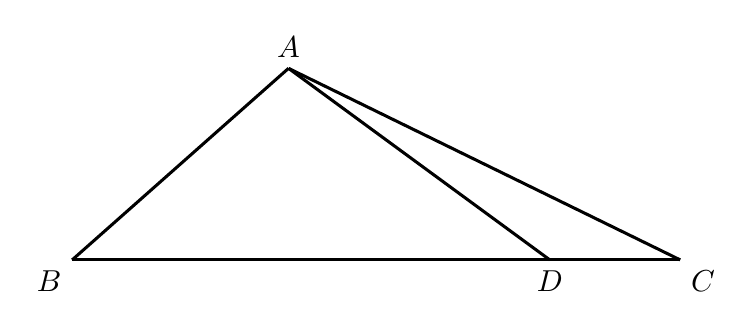
\begin{tikzpicture}[line width=1.1pt, line join=round]
% Scale s=0.009357 cm/px, origin at ink-bbox centre (464,222.5) px, y flipped
\coordinate (A) at (-1.120,1.380);   % apex (344.26,75)
\coordinate (B) at (-3.868,-1.053);  % (50.61,335)
\coordinate (C) at (3.855,-1.053);   % (876.04,335)
\coordinate (D) at (2.199,-1.053);   % (699.07,335)

% cevians and baseline (solid, black)
\draw (A) -- (B);
\draw (A) -- (C);
\draw (A) -- (D);
\draw (B) -- (C);

% labels (font from STYLE METRICS)
\node[above,font=\fontsize{10.5}{12.6}\selectfont] at (A) {$A$};
\node[below left,font=\fontsize{10.5}{12.6}\selectfont] at (B) {$B$};
\node[below,font=\fontsize{10.5}{12.6}\selectfont] at (D) {$D$};
\node[below right,font=\fontsize{10.5}{12.6}\selectfont] at (C) {$C$};
\end{tikzpicture}
\end{document}